%!Mode:: "TeX:UTF-8"
\documentclass[a4paper,11pt,UTF8]{ctexart}

\usepackage{indentfirst} %缩进
\usepackage{xeCJK}    %使用系统字体
\usepackage{fancyhdr} %自定义页眉页脚
\pagestyle{empty}                   %不设置页眉页脚
\usepackage{amsmath, amsthm, amssymb, amsfonts} %数学公式
\usepackage[a4paper,left=3cm,right=3cm,top=3cm,bottom=3cm]{geometry}
%\usepackage[tmargin=1in,bmargin=1in,lmargin=1.25in,rmargin=1.25in]{geometry}.
\usepackage{booktabs} %插入表格
\usepackage[section]{placeins} %避免浮动
\usepackage{listings} %插入代码
\usepackage{ctex}     %中文宏包
\usepackage[svgnames, table]{xcolor} %彩色表格
\usepackage{algorithm}          %伪代码
\usepackage{algorithmicx}
\usepackage{algpseudocode}
\usepackage{algorithm,algpseudocode,float}
\usepackage{lipsum}
\usepackage{enumitem}           %调整列举环境
\usepackage{url}
\usepackage{fontspec,xunicode}
\usepackage{subfigure}
\usepackage{parskip}      %m行n列图片排版方法
\defaultfontfeatures{Mapping=tex-text} %如果没有它,会有一些 tex 特殊字符无法正常使用,比如连字符。

\usepackage{graphicx}
\graphicspath{{imgs/}}

%%%%%%%%%%%%%%%%%%%%%%%%%%%%%%%%%%%%%%%%%%%%%%%%%%%%%%%%%%%%%%%%
% 缩进及行间距
%%%%%%%%%%%%%%%%%%%%%%%%%%%%%%%%%%%%%%%%%%%%%%%%%%%%%%%%%%%%%%%%
\setlength{\parindent}{22pt} %重新定义缩进长度
\setlength{\baselineskip}{20pt}  %定义行间距
%\renewcommand{\baselinestretch}{1.1} %定义行间距

%%%%%%%%%%%%%%%%%%%%%%%%%%%%%%%%%%%%%%%%%%%%%%%%%%%%%%%%%%%%%%%%
% 列表设置
%%%%%%%%%%%%%%%%%%%%%%%%%%%%%%%%%%%%%%%%%%%%%%%%%%%%%%%%%%%%%%%%
\setenumerate{fullwidth,itemindent=\parindent,listparindent=\parindent,itemsep=0ex,partopsep=0pt,parsep=0ex}
\setenumerate[2]{label=\alph*),leftmargin=1.5em}  %二级item设置
\setitemize{itemindent=38pt,leftmargin=0pt,itemsep=-0.4ex,listparindent=26pt,partopsep=0pt,parsep=0.5ex,topsep=-0.25ex}
\setdescription{itemindent=38pt,leftmargin=0pt,itemsep=-0.4ex,listparindent=26pt,partopsep=0pt,parsep=0.5ex,topsep=-0.25ex}

%%%%%%%%%%%%%%%%%%%%%%%%%%%%%%%%%%%%%%%%%%%%%%%%%%%%%%%%%%%%%%%%
% 图的标题行间距设置
%%%%%%%%%%%%%%%%%%%%%%%%%%%%%%%%%%%%%%%%%%%%%%%%%%%%%%%%%%%%%%%%
\newcommand{\bottomcaption}{%
\setlength{\abovecaptionskip}{6pt}%
\setlength{\belowcaptionskip}{6pt}%
\caption}


%%%%%%%%%%%%%%%%%%%%%%%%%%%%%%%%%%%%%%%%%%%%%%%%%%%%%%%%%%%%%%%%
% 字体定义
%%%%%%%%%%%%%%%%%%%%%%%%%%%%%%%%%%%%%%%%%%%%%%%%%%%%%%%%%%%%%%%%
\setmainfont{Times New Roman}  %默认英文字体.serif是有衬线字体sans serif无衬线字体
\setmonofont{FiraCode-Retina.ttf}
\setCJKmainfont[ItalicFont={楷体}, BoldFont={黑体}]{宋体}%衬线字体 缺省中文字体为
\setCJKsansfont{黑体}
\punctstyle{hangmobanjiao}
%-----------------------xeCJK下设置中文字体------------------------------%
\setCJKfamilyfont{song}{SimSun}                             %宋体 song
\newcommand{\song}{\CJKfamily{song}}
\setCJKfamilyfont{fs}{FangSong}                      %仿宋  fs
\newcommand{\fs}{\CJKfamily{fs}}
\setCJKfamilyfont{ktgb}{KaiTi}                      %楷体2312 ktgb
\newcommand{\ktgb}{\CJKfamily{ktgb}}
\setCJKfamilyfont{yh}{Microsoft YaHei}                    %微软雅黑 yh
\newcommand{\yh}{\CJKfamily{yh}}
\setCJKfamilyfont{hei}{SimHei}                              %黑体  hei
\newcommand{\hei}{\CJKfamily{hei}}
\setCJKfamilyfont{hwxk}{STXingkai}                                %华文行楷  hwxk
\newcommand{\hwxk}{\CJKfamily{hwxk}}
%------------------------------设置字体大小------------------------%
\newcommand{\shiyanbaogao}{\fontsize{36pt}{\baselineskip}\selectfont}
\newcommand{\chuhao}{\fontsize{42pt}{\baselineskip}\selectfont}     %初号
\newcommand{\xiaochuhao}{\fontsize{36pt}{\baselineskip}\selectfont} %小初号
\newcommand{\yihao}{\fontsize{28pt}{\baselineskip}\selectfont}      %一号
\newcommand{\erhao}{\fontsize{21pt}{\baselineskip}\selectfont}      %二号
\newcommand{\xiaoerhao}{\fontsize{18pt}{\baselineskip}\selectfont}  %小二号
\newcommand{\sanhao}{\fontsize{15.75pt}{\baselineskip}\selectfont}  %三号
\newcommand{\sihao}{\fontsize{14pt}{\baselineskip}\selectfont}       %四号
\newcommand{\xiaosihao}{\fontsize{12pt}{\baselineskip}\selectfont}  %小四号
\newcommand{\wuhao}{\fontsize{10.5pt}{\baselineskip}\selectfont}    %五号
\newcommand{\xiaowuhao}{\fontsize{9pt}{\baselineskip}\selectfont}   %小五号
\newcommand{\liuhao}{\fontsize{7.875pt}{\baselineskip}\selectfont}  %六号
\newcommand{\qihao}{\fontsize{5.25pt}{\baselineskip}\selectfont}    %七号

%%%%%%%%%%%%%%%%%%%%%%%%%%%%%%%%%%%%%%%%%%%%%%%%%%%%%%%%%%%%%%%%
% 图题字体大小相同
%%%%%%%%%%%%%%%%%%%%%%%%%%%%%%%%%%%%%%%%%%%%%%%%%%%%%%%%%%%%%%%%
\usepackage{caption}
\captionsetup{font={footnotesize}}   % footnotesize = 9pt
\captionsetup[lstlisting]{font={footnotesize}}

%%%%%%%%%%%%%%%%%%%%%%%%%%%%%%%%%%%%%%%%%%%%%%%%%%%%%%%%%%%%%%%%
% 重定义枚举编号为 1),2)...
%%%%%%%%%%%%%%%%%%%%%%%%%%%%%%%%%%%%%%%%%%%%%%%%%%%%%%%%%%%%%%%%
\renewcommand{\labelenumi}{\theenumi)}


%%%%%%%%%%%%%%%%%%%%%%%%%%%%%%%%%%%%%%%%%%%%%%%%%%%%%%%%%%%%%%%%
% 重定义section标题
%%%%%%%%%%%%%%%%%%%%%%%%%%%%%%%%%%%%%%%%%%%%%%%%%%%%%%%%%%%%%%%%
\CTEXsetup[format={\sihao\CJKfamily{zhhei}\zihao{4}},number={\chinese{section}},name={,、~},aftername={},indent={0pt},beforeskip={6pt},afterskip={6pt},format+={\flushleft}]{section}
\CTEXsetup[format={\Large\bfseries\CJKfamily{zhkai}\zihao{5}},name={(,)},number={\chinese{subsection}},aftername={},indent={22pt},beforeskip={14pt},afterskip={2pt}]{subsection}
\CTEXsetup[number={\chinese{section}},name={附录, ~~ }]{appendix}



%%%%%%%%%%%%%%%%%%%%%%%%%%%%%%%%%%%%%%%%%%%%%%%%%%%%%%%%%%%%%%%%
% 标题名称中文化
%%%%%%%%%%%%%%%%%%%%%%%%%%%%%%%%%%%%%%%%%%%%%%%%%%%%%%%%%%%%%%%%
\renewcommand\figurename{\hei 图}
\renewcommand\tablename{\hei 表}
\renewcommand\lstlistingname{\hei 代码}
\renewcommand{\algorithmicrequire}{\textbf{输入:}}
\renewcommand{\algorithmicensure}{\textbf{输出:}}
\newtheorem{define}{定义}

%%%%%%%%%%%%%%%%%%%%%%%%%%%%%%%%%%%%%%%%%%%%%%%%%%%%%%%%%%%%%%%%
% 代码设置
%%%%%%%%%%%%%%%%%%%%%%%%%%%%%%%%%%%%%%%%%%%%%%%%%%%%%%%%%%%%%%%%
\lstset{
 columns=fixed,
 numbers=left,                                        % 在左侧显示行号
 numberstyle=\tiny\color{gray},                       % 设定行号格式
 frame=single,                                      % 单线背景边框
%  frame=none,                                          % 不显示背景边框
 breaklines=true,                                     % 设定LaTeX对过长的代码行进行自动换行
 tabsize=4,                                           % 把tab扩展为4个空格,默认是8个太长
 keywordstyle=\color[RGB]{40,40,255},                 % 设定关键字颜色
 numberstyle=\footnotesize\color{darkgray}\ttfamily,
 commentstyle=\it\color[RGB]{0,96,96}\ttfamily,       % 设置代码注释的格式
 stringstyle=\rmfamily\slshape\color[RGB]{128,0,0},   % 设置字符串格式
 showstringspaces=false,                              % 不显示字符串中的空格
 language=c++,                                        % 设置语言
 basicstyle=\linespread{0.7}\xiaowuhao\ttfamily,                      % 字体字号
 morekeywords={alignas,continute,friend,register,true,alignof,decltype,goto,
 reinterpret_cast,try,asm,defult,if,return,typedef,auto,delete,inline,short,
 typeid,bool,do,int,signed,typename,break,double,long,sizeof,union,case,
 dynamic_cast,mutable,static,unsigned,catch,else,namespace,static_assert,using,
 char,enum,new,static_cast,virtual,char16_t,char32_t,explict,noexcept,struct,
 void,export,nullptr,switch,volatile,class,extern,operator,template,wchar_t,
 const,false,private,this,while,constexpr,float,protected,thread_local,
 const_cast,for,public,throw,std},
 xleftmargin=2em,
 xrightmargin=2em,
 aboveskip=1em
 %lineskip=10pt,
 %baselinestretch=1,
}

%%%%%%%%%%%%%%%%%%%%%%%%%%%%%%%%%%%%%%%%%%%%%%%%%%%%%%%%%%%%%%%%
% 伪代码分页
%%%%%%%%%%%%%%%%%%%%%%%%%%%%%%%%%%%%%%%%%%%%%%%%%%%%%%%%%%%%%%%%
\makeatletter
\renewcommand{\ALG@name}{算法}
\newenvironment{breakablealgorithm}
  {% \begin{breakablealgorithm}
   \begin{center}
     \refstepcounter{algorithm}% New algorithm
     \hrule height.8pt depth0pt \kern2pt% \@fs@pre for \@fs@ruled
     \renewcommand{\caption}[2][\relax]{% Make a new \caption
       {\raggedright\textbf{\ALG@name~\thealgorithm} ##2\par}%
       \ifx\relax##1\relax % #1 is \relax
         \addcontentsline{loa}{algorithm}{\protect\numberline{\thealgorithm}##2}%
       \else % #1 is not \relax
         \addcontentsline{loa}{algorithm}{\protect\numberline{\thealgorithm}##1}%
       \fi
       \kern2pt\hrule\kern2pt
     }
  }{% \end{breakablealgorithm}
     \kern2pt\hrule\relax% \@fs@post for \@fs@ruled
   \end{center}
  }
\makeatother



\begin{document}
\xiaosihao\song

\begin{titlepage}
\center{\yihao{\hwxk{南京航空航天大学}}}
\vspace{6cm}
\center{\shiyanbaogao{\ktgb{上~机~实~验~报~告}}}
\vspace{4cm}

\begin{center}
\begin{large}
\begin{tabular}{rc}
  \xiaoerhao{\hei{课\qquad 程}}& \hspace{1.7cm}\xiaoerhao{\hei{数据结构\hspace{1.7cm}}} \\
  \cline{2-2}\\
  \xiaoerhao{\hei{班\qquad 级}}& \hspace{1.7cm}\xiaoerhao{\hei{1819001\hspace{1.7cm}}} \\
  \cline{2-2}\\
  \xiaoerhao{\hei{学\qquad 号}}& \hspace{1.7cm}\xiaoerhao{\hei{161940233\hspace{1.7cm}}} \\
  \cline{2-2}\\
  \xiaoerhao{\hei{姓\qquad 名}}& \xiaoerhao{\hei{颜~宇~明}}\\
  \cline{2-2}\\
  \xiaoerhao{\hei{指导教师}}& \xiaoerhao{\hei{秦~小~麟}}\\
  \cline{2-2}
\end{tabular}
\end{large}
\end{center}
\vfill \hfill
\end{titlepage}
\clearpage


\tableofcontents
\newpage
\section{Lab1}
\subsection{数据结构}
链表,顺序表
\subsection{算法设计思想}

主要描述插入操作与删除操作的思路

\subsection{源程序}

\begin{lstlisting}[caption=1Linked\_list.cpp,captionpos=b]
#include <malloc.h>
#include <stdio.h>
class ADT_list{
public:
    typedef struct node
    {
        int value;
        struct node *next;
    } node;

    node *head;
    int length = -1;

    void InitLIst(){
        node *tmp = (node *)malloc(sizeof(node));
        length = 0;
        head = tmp;
        tmp->next = NULL;
    }
    void DestoryList(){
        node *p, *temp;
        p = head;
        while (p != NULL){
            temp = p;
            p = p->next;
            free(temp);
        }
        length = -1;
    }
    void ClearList(){
        node *p, *temp;
        p = head->next;
        while (p != NULL){
            temp = p;
            p = p->next;
            free(temp);
        }
        length = 0;
    }
    bool ListEmpty(){
        if (length < 1) return true;
        return false;
    }
    int ListLength(){
        return length;
    }
    int GetElem(int index){
        node *p;
        int i = 0;
        p = head->next;
        while (p != NULL){
            if (index == ++i)
                return p->value;
            p = p->next;
        }
        return 0;
    }
    int LocateElem(int num){
        node *p;
        p = head->next;
        int index = 0;
        while (p != NULL){
            if (p->value == num)
                return index;
            p = p->next;
            index++;
        }
        return -1;
    }
    int PriorElem(int cur_num){
        node *p, *temp;
        p = head->next;
        while (p != NULL){
            temp = p;
            p = p->next;
            if (p != NULL && p->value == cur_num)
                return temp->value;
        }
        return 0;
    }
    int NextElem(int cur_num){
        node *p, *temp;
        p = head->next;
        while (p != NULL){
            temp = p;
            p = p->next;
            if (p != NULL && temp->value == cur_num)
                return p->value;
        }
        return NULL;
    }
    void ListTraverse(){
        node *p;
        p = head->next;
        while (p != NULL){
            printf("%d ", p->value);
            p = p->next;
        }
        printf("\n");
    }
    int SetElem(int index, int num){
        node *p;
        int i = 0;
        p = head->next;
        while (p != NULL){
            if (index != i++) {
                p = p->next;
                continue;
            }
            int old = p->value;
            p->value = num;
            return old;
        }
        return 0;
    }
    void InsertElem(int index, int num){
        node *p, *temp;
        int i = 0;
        p = head;
        length++;
        while (p != NULL){
            if (index != ++i) {
                temp = p;
                p = p->next;
                continue;
            }
            temp = p->next;
            node *tmp = (node *)malloc(sizeof(node));
            p->next = tmp;
            tmp->next = temp;
            tmp->value = num;
            return;
        }
        node *tmp = (node *)malloc(sizeof(node));
        temp->next = tmp;
        tmp->value = num;
        tmp->next = NULL;
    }
    void DeleteElem(int index){
        node *p, *temp;
        int i = 0;
        temp = head;
        p = head->next;
        length--;
        while (p != NULL){
            if (index != ++i) {
                temp = p;
                p = p->next;
                continue;
            }
            temp->next = p->next;
            free(p);
        }
    }
} ADTlist;

int main(){
    ADTlist.InitLIst();
    ADTlist.InsertElem(1, 1);
    ADTlist.InsertElem(2, 1);
    ADTlist.InsertElem(3, 3);
    ADTlist.InsertElem(4, 3);
    ADTlist.InsertElem(5, 3);
    ADTlist.InsertElem(6, 4);
    ADTlist.InsertElem(7, 5);
    ADTlist.ListTraverse();
    ADTlist.SetElem(2, 7);
    printf("%d\n", ADTlist.NextElem(1));
    ADTlist.ListTraverse();
    ADTlist.DestoryList();
}
\end{lstlisting}

\begin{lstlisting}[caption=1Sequence\_list.cpp,captionpos=b]
#include <stdio.h>
class ADT_list{
public:
    int list[999];
    int rear = -1;
    void InitLIst(){
        rear++;
    }
    void DestoryList(){
        rear = -1;
    }
    void ClearList(){
        for(int i = 0; i <= rear; i++){
            list[i] = 0;
        }
    }
    bool ListEmpty(){
        if (rear == 0 && list[rear] == 0){
            return true;
        }
        return false;
    }
    int ListLength(){
        return rear;
    }
    int GetElem(int num){
        return *(list + num);
    }
    int LocateElem(int num){
        for (int i = 0; i < rear; i++){
            if (list[i] == num){
                return i;
            }
        }
        return -1;
    }
    int PriorElem(int cur_num){
        int pre;
        for (int i = 0; i < rear; i++){
            if (list[i] == cur_num){
                return i - 1;
            }
        }
        return -1;
    }
    int NextElem(int cur_num){
        for (int i = 0; i < rear; i++){
            if (list[i] == cur_num && i != rear){
                return i + 1;
            }
        }
        return -1;
    }
    void ListTraverse(){
        for (int i = 0; i < rear; i++){
            printf("%d ", list[i]);
        }
        printf("\n");
    }
    int SetElem(int index, int num){
        list[index] = num;
        return num = list[index];
    }
    void InsertElem(int index, int num){
        rear++;
        for (int i = rear; i > index - 1; i--){
            list[i] = list[i - 1];
        }
        list[index - 1] = num;
    }
    void DeleteElem(int index){
        for (int i = index - 1; i < rear; i++){
            list[i] = list[i + 1];
        }
        rear--;
    }
} ADTlist;
\end{lstlisting}

\begin{lstlisting}[caption=2Linked\_list\_Reverse.cpp,captionpos=b]
  #include<stdio.h>
  #include <malloc.h>

  class ADT_list{
  public:
      typedef struct node
      {
          int value;
          struct node *next;
      } node;

      node *head;
      int length = -1;

      void InitLIst(){
          node *tmp = (node *)malloc(sizeof(node));
          length = 0;
          head = tmp;
          tmp->next = NULL;
      }
      void DestoryList(){
          node *p, *temp;
          p = head;
          while (p != NULL){
              temp = p;
              p = p->next;
              free(temp);
          }
          length = -1;
      }
      void ClearList(){
          node *p, *temp;
          p = head->next;
          while (p != NULL){
              temp = p;
              p = p->next;
              free(temp);
          }
          length = 0;
      }
      bool ListEmpty(){
          if (length < 1) return true;
          return false;
      }
      int ListLength(){
          return length;
      }
      int GetElem(int index){
          node *p;
          int i = 0;
          p = head->next;
          while (p != NULL){
              if (index == ++i)
                  return p->value;
              p = p->next;
          }
          return 0;
      }
      int LocateElem(int num){
          node *p;
          p = head->next;
          int index = 0;
          while (p != NULL){
              if (p->value == num)
                  return index;
              p = p->next;
              index++;
          }
          return -1;
      }
      int PriorElem(int cur_num){
          node *p, *temp;
          p = head->next;
          while (p != NULL){
              temp = p;
              p = p->next;
              if (p != NULL && p->value == cur_num)
                  return temp->value;
          }
          return 0;
      }
      int NextElem(int cur_num){
          node *p, *temp;
          p = head->next;
          while (p != NULL){
              temp = p;
              p = p->next;
              if (p != NULL && temp->value == cur_num)
                  return p->value;
          }
          return 0;
      }
      void ListTraverse(){
          node *p;
          p = head->next;
          while (p != NULL){
              printf("%d ", p->value);
              p = p->next;
          }
          printf("\n");
      }
      int SetElem(int index, int num){
          node *p;
          int i = 0;
          p = head->next;
          while (p != NULL){
              if (index != i++) {
                  p = p->next;
                  continue;
              }
              int old = p->value;
              p->value = num;
              return old;
          }
          return 0;
      }
      void InsertElem(int index, int num){
          node *p, *temp;
          int i = 0;
          p = head;
          length++;
          while (p != NULL){
              if (index != ++i) {
                  temp = p;
                  p = p->next;
                  continue;
              }
              temp = p->next;
              node *tmp = (node *)malloc(sizeof(node));
              p->next = tmp;
              tmp->next = temp;
              tmp->value = num;
              return;
          }
          node *tmp = (node *)malloc(sizeof(node));
          temp->next = tmp;
          tmp->value = num;
          tmp->next = NULL;
      }
      void DeleteElem(int index){
          node *p, *temp;
          int i = 0;
          temp = head;
          p = head->next;
          length--;
          while (p != NULL){
              if (index != ++i) {
                  temp = p;
                  p = p->next;
                  continue;
              }
              temp->next = p->next;
              free(p);
          }
      }
      void Reverse(){
          if (length < 1) return;
          node *p, *temp, *tmp = NULL;
          temp = p = head->next;
          while(temp != NULL){
              temp = p->next;
              p->next = tmp;
              tmp = p;
              p = temp;
          }
          head->next = tmp;
      }
  } ADTlist;

  int main(){
      ADTlist.InitLIst();
      ADTlist.InsertElem(1, 1);
      ADTlist.InsertElem(2, 2);
      ADTlist.InsertElem(3, 3);
      ADTlist.InsertElem(4, 4);
      ADTlist.ListTraverse();
      ADTlist.Reverse();
      ADTlist.ListTraverse();
      ADTlist.DestoryList();
  }
\end{lstlisting}

\begin{lstlisting}[caption=2Sequence\_list\_Reverse.cpp,captionpos=b]
  #include<stdio.h>
  int list[3] = {1, 2, 3};
  void Reverse(int list[], int length){
      length--;
      for ( int i = 0; i < length; i++){
          int temp = list[i];
          list[i] = list[length - i];
          list[length - i] = temp;
      }
  }

  int main(){
      int length = 3;
      Reverse(list, length);
      for( int i = 0; i < length; i++){
          printf("%d ", list[i]);
      }
  }
\end{lstlisting}

\begin{lstlisting}[caption=3Linked\_list\_Remove.cpp,captionpos=b]
  #include <malloc.h>
  #include <stdio.h>
  class ADT_list{
  public:
      typedef struct node
      {
          int value;
          struct node *next;
      } node;

      node *head;
      int length = -1;

      void InitLIst(){
          node *tmp = (node *)malloc(sizeof(node));
          length = 0;
          head = tmp;
          tmp->next = NULL;
      }
      void DestoryList(){
          node *p, *temp;
          p = head;
          while (p != NULL){
              temp = p;
              p = p->next;
              free(temp);
          }
          length = -1;
      }
      void ClearList(){
          node *p, *temp;
          p = head->next;
          while (p != NULL){
              temp = p;
              p = p->next;
              free(temp);
          }
          length = 0;
      }
      bool ListEmpty(){
          if (length < 1) return true;
          return false;
      }
      int ListLength(){
          return length;
      }
      int GetElem(int index){
          node *p;
          int i = 0;
          p = head->next;
          while (p != NULL){
              if (index == ++i)
                  return p->value;
              p = p->next;
          }
          return 0;
      }
      int LocateElem(int num){
          node *p;
          p = head->next;
          int index = 0;
          while (p != NULL){
              if (p->value == num)
                  return index;
              p = p->next;
              index++;
          }
          return -1;
      }
      int PriorElem(int cur_num){
          node *p, *temp;
          p = head->next;
          while (p != NULL){
              temp = p;
              p = p->next;
              if (p != NULL && p->value == cur_num)
                  return temp->value;
          }
          return 0;
      }
      int NextElem(int cur_num){
          node *p, *temp;
          p = head->next;
          while (p != NULL){
              temp = p;
              p = p->next;
              if (p != NULL && temp->value == cur_num)
                  return p->value;
          }
          return 0;
      }
      void ListTraverse(){
          node *p;
          p = head->next;
          while (p != NULL){
              printf("%d ", p->value);
              p = p->next;
          }
          printf("\n");
      }
      int SetElem(int index, int num){
          node *p;
          int i = 0;
          p = head->next;
          while (p != NULL){
              if (index != i++) {
                  p = p->next;
                  continue;
              }
              int old = p->value;
              p->value = num;
              return old;
          }
          return 0;
      }
      void InsertElem(int index, int num){
          node *p, *temp;
          int i = 0;
          p = head;
          length++;
          while (p != NULL){
              if (index != ++i) {
                  temp = p;
                  p = p->next;
                  continue;
              }
              temp = p->next;
              node *tmp = (node *)malloc(sizeof(node));
              p->next = tmp;
              tmp->next = temp;
              tmp->value = num;
              return;
          }
          node *tmp = (node *)malloc(sizeof(node));
          temp->next = tmp;
          tmp->value = num;
          tmp->next = NULL;
      }
      void DeleteElem(int index){
          node *p, *temp;
          int i = 0;
          temp = head;
          p = head->next;
          length--;
          while (p != NULL){
              if (index != ++i) {
                  temp = p;
                  p = p->next;
                  continue;
              }
              temp->next = p->next;
              free(p);
          }
      }
      void Remove(){
          node *p = head->next, *temp = head;
          int use[999] = {0};
          while (p != NULL){
              if (use[p->value]) {
                  temp->next = p->next;
                  free(p);
                  length--;
                  p = temp->next;
                  continue;
              }
              use[p->value] = 1;
              temp = p;
              p = p->next;
          }
      }
  } ADTlist;

  int main(){
      ADTlist.InitLIst();
      ADTlist.InsertElem(1, 1);
      ADTlist.InsertElem(2, 1);
      ADTlist.InsertElem(3, 3);
      ADTlist.InsertElem(4, 3);
      ADTlist.InsertElem(5, 3);
      ADTlist.InsertElem(6, 4);
      ADTlist.InsertElem(7, 4);
      ADTlist.ListTraverse();
      ADTlist.Remove();
      ADTlist.ListTraverse();
      ADTlist.DestoryList();
  }
\end{lstlisting}

\begin{lstlisting}[caption=3Sequence\_list\_Remove.cpp,captionpos=b]
  #include <stdio.h>
  class ADT_list{
  public:
      int list[999];
      int rear = -1;
      void InitLIst(){
          rear++;
      }
      void DestoryList(){
          rear = -1;
      }
      void ClearList(){
          for(int i = 0; i <= rear; i++){
              list[i] = 0;
          }
      }
      bool ListEmpty(){
          if (rear == 0 && list[rear] == 0){
              return true;
          }
          return false;
      }
      int ListLength(){
          return rear;
      }
      int GetElem(int num){
          return *(list + num);
      }
      int LocateElem(int num){
          for (int i = 0; i < rear; i++){
              if (list[i] == num){
                  return i;
              }
          }
          return -1;
      }
      int PriorElem(int cur_num){
          int pre;
          for (int i = 0; i < rear; i++){
              if (list[i] == cur_num){
                  return i - 1;
              }
          }
          return -1;
      }
      int NextElem(int cur_num){
          for (int i = 0; i < rear; i++){
              if (list[i] == cur_num && i != rear){
                  return i + 1;
              }
          }
          return -1;
      }
      void ListTraverse(){
          for (int i = 0; i < rear; i++){
              printf("%d ", list[i]);
          }
          printf("\n");
      }
      int SetElem(int index, int num){
          list[index] = num;
          return num = list[index];
      }
      void InsertElem(int index, int num){
          rear++;
          for (int i = rear; i > index - 1; i--){
              list[i] = list[i - 1];
          }
          list[index - 1] = num;
      }
      void DeleteElem(int index){
          for (int i = index - 1; i < rear; i++){
              list[i] = list[i + 1];
          }
          rear--;
      }
      void Remove(){
          int use[999];
          for (int i = 0; i < rear; i++){
              if (use[list[i]]){
                  DeleteElem(i + 1);
                  i--;
                  continue;
              }
              use[list[i]] = 1;
              i++;
          }
      }
  } ADTlist;

  int main(){
      ADTlist.InitLIst();
      ADTlist.InsertElem(1, 1);
      ADTlist.InsertElem(1, 1);
      ADTlist.InsertElem(2, 2);
      ADTlist.InsertElem(2, 2);
      ADTlist.InsertElem(3, 3);
      ADTlist.InsertElem(3, 3);
      ADTlist.InsertElem(3, 3);
      ADTlist.InsertElem(4, 4);
      ADTlist.InsertElem(4, 4);
      ADTlist.InsertElem(4, 4);
      ADTlist.ListTraverse();
      ADTlist.Remove();
      ADTlist.ListTraverse();
      ADTlist.DestoryList();
  }

\end{lstlisting}

\begin{lstlisting}[caption=4CSP.cpp,captionpos=b]
  #include <stdio.h>
  int n, m, l, a[255555], num, h[333];
  int main(){
      freopen("4CSP1", "r", stdin);
      scanf("%d%d%d", &n, &m, &l);
      while (scanf("%d", &a[num]) != EOF) num++;
      for (int i = 0; i < n; i++)
      for (int j = 0; j < m; j++)
          h[a[i * m + j]]++;
      for (int i = 0; i < l; i++)
          printf("%d ", h[i]);
  }
\end{lstlisting}

\begin{lstlisting}[caption=5CSP.cpp,captionpos=b]
  #include <stdio.h>
  #include <algorithm>
  int n, l, t, a[999], num, speed[999], use[999];
  int main(){
      freopen("5CSP1", "r", stdin);
      scanf("%d%d%d", &n, &l, &t);
      while (scanf("%d", &a[num]) != EOF) num++;
      std::fill(speed, speed + 999, 1);
      while(t--){
          std::fill(use, use + 999, -1);
          for (int j = 0; j < n; j++){
              a[j] += speed[j];
              if (a[j] == l || a[j] == 0) speed[j] *= -1;
              if(use[a[j]] >= 0) speed[j] *= -1, speed[use[a[j]]] *= -1;
              else use[a[j]] = j;
          }
      }
      for (int i = 0; i < n; i++)
          printf("%d ", a[i]);
  }
\end{lstlisting}

\subsection{测试数据及其结果}

\begin{lstlisting}[caption=1Linked\_list.cpp,captionpos=b]
    1 1 3 3 3 4 5
    1
    1 1 7 3 3 4 5
\end{lstlisting}

\begin{lstlisting}[caption=2Linked\_list\_Reverse.cpp,captionpos=b]
    1 2 3 4
    4 3 2 1
\end{lstlisting}

\begin{lstlisting}[caption=2Sequence\_list\_Reverse.cpp,captionpos=b]
    3 2 1
\end{lstlisting}

\begin{lstlisting}[caption=3Linked\_list\_Remove.cpp,captionpos=b]
    1 1 3 3 3 4 4
    1 3 4
\end{lstlisting}

\begin{lstlisting}[caption=3Sequence\_list\_Remove.cpp,captionpos=b]
    1 2 3 4 4 4 3 3 2 1
    1 2 3 4
\end{lstlisting}

\begin{lstlisting}[caption=4CSP.cpp,captionpos=b]
    1 1 1 1 1 1 1 1 1 1 1 1 1 1 1 1
\end{lstlisting}

\begin{lstlisting}[caption=5CSP.cpp,captionpos=b]
    7 9 9
\end{lstlisting}

\subsection{时间复杂度}

数组实现\par
\begin{enumerate}
    \item 插入元素: $$O(n)$$
    \item 删除元素:$$O(n)$$
\end{enumerate}\par

链表实现\par

\begin{enumerate}
    \item 插入元素: $$O(1)$$
    \item 删除元素:$$O(n)$$
\end{enumerate}\par

\subsection{改进方法}
链表的基本操作,不需要改进。



\section{Lab2}
\subsection{数据结构}
链表,顺序表
\subsection{算法设计思想}
主要描述插入操作与删除操作的思路
\subsection{源程序}

\lstinputlisting[caption=1Linked\_list\_sort.cpp,captionpos=b]{../lab2/1Linked_list_sort.cpp}
\lstinputlisting[caption=1Sequence\_list\_sort.cpp,captionpos=b]{../lab2/1Sequence_list_sort.cpp}
\lstinputlisting[caption=2Linked\_list\_union.cpp,captionpos=b]{../lab2/2Linked_list_union.cpp}
\lstinputlisting[caption=3Linked\_list\_Josephus.cpp,captionpos=b]{../lab2/3Linked_list_Josephus.cpp}
\lstinputlisting[caption=3Sequence\_list\_Josephus.cpp,captionpos=b]{../lab2/3Sequence_list_Josephus.cpp}
\lstinputlisting[caption=4CSP.cpp,captionpos=b]{../lab2/4CSP.cpp}
\lstinputlisting[caption=5CSP.cpp,captionpos=b]{../lab2/5CSP.cpp}
\lstinputlisting[caption=Linked\_list.cpp,captionpos=b]{../lab2/Linked_list.cpp}
\lstinputlisting[caption=Linked\_list.h,captionpos=b]{../lab2/Linked_list.h}
\lstinputlisting[caption=Sequence\_list.cpp,captionpos=b]{../lab2/Sequence_list.cpp}
\lstinputlisting[caption=Sequence\_list.h,captionpos=b]{../lab2/Sequence_list.h}

\subsection{测试数据及其结果}

\begin{lstlisting}[caption=1Linked\_list\_sort.cpp,captionpos=b]
    3 5 1 2 6 7 0
    0 1 2 3 5 6 7
\end{lstlisting}

\begin{lstlisting}[caption=1Sequence\_list\_sort.cpp,captionpos=b]
    3 5 1 2 6 7 0
    0 1 2 3 5 6 7
\end{lstlisting}

\begin{lstlisting}[caption=2Sequence\_list\_union.cpp,captionpos=b]
    7 6 5 4 3 2 0
    9 8 7 6 3 2 1
    7 6 3 2
\end{lstlisting}

\begin{lstlisting}[caption=3Linked\_list\_Josephus.cpp,captionpos=b]
    3 6 2 7 5 1 4
\end{lstlisting}

\begin{lstlisting}[caption=3Sequence\_list\_Josephus.cpp,captionpos=b]
    2 4 6 1 5 3 7
\end{lstlisting}

\begin{lstlisting}[caption=4CSP.cpp,captionpos=b]
5
\end{lstlisting}
\begin{lstlisting}[caption=5CSP.cpp,captionpos=b]
3
\end{lstlisting}

\subsection{时间复杂度}
数组实现\par
\begin{enumerate}
    \item 插入元素: $$O(n)$$
    \item 删除元素:$$O(n)$$
\end{enumerate}\par

链表实现\par

\begin{enumerate}
    \item 插入元素: $$O(1)$$
    \item 删除元素:$$O(n)$$
\end{enumerate}\par

\subsection{改进方法}
可以尝试用一行代码解决约瑟夫问题。

\section{Lab3}
\subsection{数据结构}
链表,顺序表
\subsection{算法设计思想}
主要描述插入操作与删除操作的思路。\par

按行摆放,在确定一个皇后应该摆的列时,需要检查当前列是否合法,如果合法,则将皇后放置在当前位置,并进行递归,回溯。每行都摆满皇后时,则产生了一种解法,将所有解法收集并返回。\par
合法性判断方法:当前将要摆放皇后的位置和其他已摆放皇后的位置不能在同一列,且不能在同一条斜线上。这里判断是否在同一条斜线上可以通过两个皇后的位置横坐标之差和纵坐标之差的绝对值是否相等来判断。\par
\subsection{源程序}

\lstinputlisting[caption=3Eight\_Queens.cpp,captionpos=b]{../lab3/3Eight_Queens.cpp}
\lstinputlisting[caption=4CSP.cpp,captionpos=b]{../lab3/4CSP.cpp}
\lstinputlisting[caption=5CSP.cpp,captionpos=b]{../lab3/5CSP.cpp}
\lstinputlisting[caption=5Linked\_list.cpp,captionpos=b]{../lab3/5Linked_list.cpp}
\lstinputlisting[caption=5Linked\_list.h,captionpos=b]{../lab3/5Linked_list.h}

\subsection{测试数据及其结果}

\begin{lstlisting}[caption=3Eight\_Queens.cpp,captionpos=b]
    0 4 7 5 2 6 1 3
\end{lstlisting}

\begin{lstlisting}[caption=4CSP.cpp,captionpos=b]
    100000000
\end{lstlisting}

\begin{lstlisting}[caption=5CSP.cpp,captionpos=b]
    2
    1
    1
    IGNORED
\end{lstlisting}

\subsection{时间复杂度}
$$O(n^2)$$
\subsection{改进方法}
可以尝试把八皇后扩展到n皇后。


\section{Lab4}
\subsection{数据结构}
三元组
\subsection{算法设计思想}
遍历两次把行和列换一下,最后完成转置。
\subsection{源程序}

\lstinputlisting[caption=1triple.cpp,captionpos=b]{../lab4/1triple.cpp}
\lstinputlisting[caption=2Saddle\_point.cpp,captionpos=b]{../lab4/2Saddle_point.cpp}
\lstinputlisting[caption=3CSP.cpp,captionpos=b]{../lab4/3CSP.cpp}
\lstinputlisting[caption=4CSP.cpp,captionpos=b]{../lab4/4CSP.cpp}

\subsection{测试数据及其结果}

\begin{lstlisting}[caption=1triple.cpp,captionpos=b]
    0 2 4
    1 1 6
    3 0 5
    3 4 3
    4 2 7
\end{lstlisting}

\begin{lstlisting}[caption=2Saddle\_point.cpp,captionpos=b]
    25
\end{lstlisting}

\begin{lstlisting}[caption=3CSP.cpp,captionpos=b]
    46
\end{lstlisting}
\begin{lstlisting}[caption=4CSP.cpp,captionpos=b]
1 2
6 7 8 9 10
11 12 13 14
3 4
\end{lstlisting}







\subsection{时间复杂度}
$$O(n)$$


\section{Lab5}
\subsection{数据结构}
二叉树
\subsection{算法设计思想}
二叉树的基本操作,插入,删除。
\subsection{源程序}

\lstinputlisting[caption=,captionpos=b]{../lab5/1BinaryTree.cpp}
\lstinputlisting[caption=,captionpos=b]{../lab5/1BinaryTree.h}
\lstinputlisting[caption=,captionpos=b]{../lab5/2Nonrecursive.cpp}
\lstinputlisting[caption=,captionpos=b]{../lab5/3delete.cpp}
\lstinputlisting[caption=,captionpos=b]{../lab5/4Complete_binary_tree.cpp}
\lstinputlisting[caption=,captionpos=b]{../lab5/5CSP.cpp}

\subsection{测试数据及其结果}

\begin{lstlisting}[caption=2Nonrecursive.cpp,captionpos=b]
    ABDHIECFJG
    ABDHIECFJG
    HDIBEAFJCG
    HDIBEAFJCG
    HIDEBJFGCA
    HIDEBJFGCA
    ABCDEFGHIJ
\end{lstlisting}

\begin{lstlisting}[caption=3delete.cpp,captionpos=b]
    ABDHIECFJG
    ABECFJG
\end{lstlisting}

\begin{lstlisting}[caption=4Complete\_binary\_tree.cpp,captionpos=b]
    1
\end{lstlisting}

\subsection{时间复杂度}
$$O(log_{2}n)$$

\section{Lab6}
\subsection{数据结构}
图,孩子兄弟表示法,二叉树
\subsection{算法设计思想}
构建哈夫曼树,孩子兄弟表示法就是把二叉树稍微改一改。
\subsection{源程序}
\lstinputlisting[caption=,captionpos=b]{../lab6/1Graph.cpp}
\lstinputlisting[caption=,captionpos=b]{../lab6/1Graph.h}
\lstinputlisting[caption=,captionpos=b]{../lab6/2HuffmanTree.cpp}
\lstinputlisting[caption=,captionpos=b]{../lab6/3BinaryTree.cpp}
\lstinputlisting[caption=,captionpos=b]{../lab6/3BinaryTree.h}
\lstinputlisting[caption=,captionpos=b]{../lab6/3BinaryTreeweigh.cpp}
\lstinputlisting[caption=,captionpos=b]{../lab6/4Kidbrother.cpp}
\lstinputlisting[caption=,captionpos=b]{../lab6/4Kidbrother.h}
\lstinputlisting[caption=,captionpos=b]{../lab6/4Outputelement.cpp}
\lstinputlisting[caption=,captionpos=b]{../lab6/5CSP.cpp}

\subsection{测试数据及其结果}
\begin{lstlisting}[caption=4Outputelement.cpp,captionpos=b]
    ABDHIECFJG
    \--> A
      |--> B
      | |--> D
      | | |--> H
      | | \--> I
      | \--> E
      \--> C
        |--> F
        | \--> J
        \--> G
    A C G
    B E F J
    D I
    H
\end{lstlisting}

\begin{lstlisting}[caption=3BinaryTreeweigh.cpp,captionpos=b]
    \--> A
    |--> B
    | |--> D
    | | |--> H
    | | \--> I
    | \--> E
    \--> C
      |--> F
      | \--> J
      \--> G
  4
\end{lstlisting}

\begin{lstlisting}[caption=2HuffmanTree.cpp,captionpos=b]
    \--> 100
    |--> 42
    | |--> 19
    | | |--> 8
    | | | |--> 3
    | | | \--> 5
    | | \--> 11
    | \--> 23
    \--> 58
      |--> 29
      \--> 29
        |--> 14
        \--> 15
          |--> 7
          \--> 8
\end{lstlisting}

\begin{lstlisting}[caption=5CSP.cpp,captionpos=b]
    0 0 0 0 0 0 0 0 0 0
    0 0 0 0 0 0 0 0 0 0
    0 0 0 0 0 0 0 0 0 0
    0 0 0 0 0 0 0 0 0 0
    0 0 0 0 0 0 0 0 0 0
    0 0 0 0 0 0 0 0 0 0
    0 0 0 0 0 0 0 0 0 0
    0 0 0 0 0 0 0 0 0 0
    0 0 0 0 0 0 0 0 0 0
    0 0 0 0 0 0 0 0 0 0
    0 0 0 0 0 0 0 1 0 0
    0 0 0 0 0 0 1 0 0 0
    0 0 0 0 0 0 1 0 0 0
    1 1 1 1 1 1 1 1 1 1
    0 0 0 0 1 1 0 0 0 0
\end{lstlisting}


\section{Lab7}
\subsection{数据结构}
广度优先搜索,深度优先搜索,Dijkstra算法
\subsection{算法设计思想}
广度优先搜索,深度优先搜索,Dijkstra算法的基本思想

\subsection{源程序}
\lstinputlisting[caption=,captionpos=b]{../lab7/1BFS.cpp}
\lstinputlisting[caption=,captionpos=b]{../lab7/1DFS.cpp}
\lstinputlisting[caption=,captionpos=b]{../lab7/1Graph.cpp}
\lstinputlisting[caption=,captionpos=b]{../lab7/1Graph.h}
\lstinputlisting[caption=,captionpos=b]{../lab7/2Dijkstra.cpp}
\lstinputlisting[caption=,captionpos=b]{../lab7/3CSP.cpp}
\lstinputlisting[caption=,captionpos=b]{../lab7/4CSP.cpp}
\subsection{测试数据及其结果}
\begin{lstlisting}[caption=1DFS.cpp,captionpos=b]
    1 3 7 6 2 4 5
\end{lstlisting}
\begin{lstlisting}[caption=1BFS.cpp,captionpos=b]
    1 3 7 6 2 4 5
\end{lstlisting}
\begin{lstlisting}[caption=2Dijkstra.cpp,captionpos=b]
    0 1 1 2 3 2
\end{lstlisting}
\begin{lstlisting}[caption=3CSP.cpp,captionpos=b]
    222 1 0
\end{lstlisting}
\begin{lstlisting}[caption=4CSP.cpp,captionpos=b]
    6
\end{lstlisting}

\section{Lab8}
\subsection{数据结构}
\subsection{算法设计思想}
\subsection{源程序}
\subsection{测试数据及其结果}
\begin{lstlisting}[caption=1BinarySortTree.cpp,captionpos=b]
    \--> 62
    |--> 58
    | |--> 47
    |   |--> 35
    |   | |--> 29
    |   | \--> 37
    |   |   |--> 36
    |   \--> 51
    |     |--> 49
    |     | |--> 48
    |     | \--> 50
    |     \--> 56
    \--> 88
      |--> 73
      \--> 99
        |--> 93
  \--> 62
    |--> 58
    | |--> 37
    |   |--> 35
    |   | |--> 29
    |   | \--> 36
    |   \--> 51
    |     |--> 49
    |     | |--> 48
    |     | \--> 50
    |     \--> 56
    \--> 88
      |--> 73
      \--> 99
        |--> 93
\end{lstlisting}
所有的排序结果都是:
\begin{lstlisting}[caption=,captionpos=b]
    62 58 88 47 73 99 35 51 93 29 37 49 56 36 48 50
    29 35 36 37 47 48 49 50 51 56 58 62 73 88 93 99
\end{lstlisting}

\begin{lstlisting}[caption=5CSP.cpp,captionpos=b]
    0 0
    1 2
    2 1
    3 0
    4 0
\end{lstlisting}

\subsection{时间复杂度}
\begin{figure}[htbp] % h为当前位置,!htb为忽略美学标准,htbp为浮动图形
    \centering
    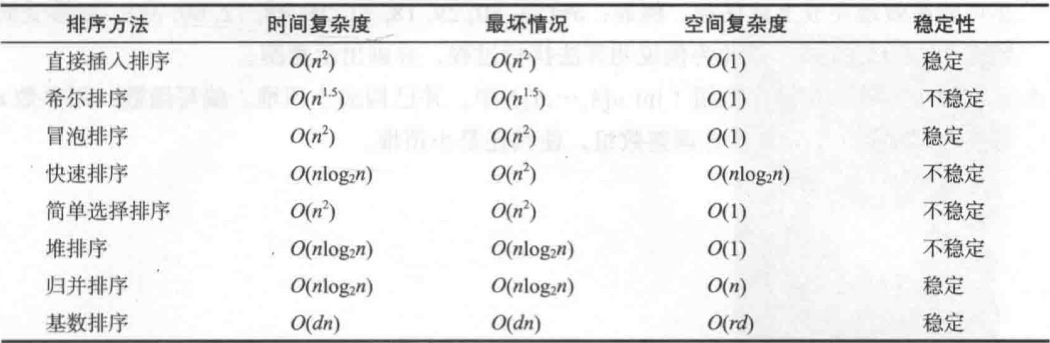
\includegraphics[width=12cm]{1.jpg}
    \caption{实验截图}
\end{figure}

\setlength{\parskip}{6pt}  %定义段间距
\vspace{4cm}
\end{document}